\chapter{Introduction aux Christologies au défi de la culture pluraliste}
\mn{Xavier Gué Cours ISTR 2022-2023}
\section{Synthèse du cours « Christologies et cultures dans l’histoire »}
\subsection{Prolégomènes à une réflexion sur la relation entre les christologies et les cultures et
les religions}

 \begin{Synthesis}
 Prolégomène : 
 \begin{itemize}
     \item  Un écart entre Jésus historique et la possibilité pour nous d'y accéder 
     \item un moment spécifique : la canonisation des Ecritures, reçues par la communauté. 
 \end{itemize}

 \end{Synthesis}

 
\paragraph{Passage}
 Jésus annonce le Règne de Dieu et les premiers disciples annoncent le Christ.

 \paragraph{Mystère pascal} Jésus passe d'un homme singulier au Christ qui est pour tous les hommes, qui est Un avec Dieu. A partir de ce moment là, il devient une bonne nouvelle pour tous les hommes, car il nous permet d'être uni à Dieu et avec tous les hommes.


\paragraph{Comment ?} La transmission du mystère du Christ se joue de manière \textit{vitale} (style de vie des disciples) et en même temps le discours du \textit{discours} (Christologie). Comment le discours sur Jésus va transmettre Jésus dans l'histoire : d'abord les juifs, puis le monde grec, le monde romain,... A chaque fois, des mondes très différents.

\begin{Synthesis}
    Si on affirme que Jésus est pour tous les hommes et tous les temps, il faut qu'on puisse l'annoncer et qu'il soit reçu dans tous les temps et toutes les cultures.
\end{Synthesis}


\paragraph{Christologie doit vérifier l'universalité du Christ} Vérifier : attester. En assumant la \textit{matrice de chaque culture}, le Christ se fera comprendre et recevoir. Rejoindre tous les hommes là où ils sont dans leur culture. 

\paragraph{Une partie résiste} Il s'agit de purifier la culture qui reçoit par le Christ

\paragraph{la Révélation se déploie dans l'histoire par la rencontre avec les Cultures} Tout dialogue transforme. Pas slt un développment organique dans l'histoire mais des influences qui viennent de l'extérieur de l'Eglise. Vincent de Lerins pense une vision organique de l'Eglise mais il y a un échange organique avec l'autre.

\paragraph{la rencontre avec l'autre} a pu développer des hérésies mais aussi développer une théologie féconde, de plus indispensable. 
Règle de discernement et de foi qui permet de vérifier : Calcédoine dit ce qu'on ne peut pas dire. La foi interprétant les Ecritures.

\paragraph{le Christ continue à s'incarner aujourd'hui} la parole de Dieu à s'incarner de nouveau d'une certaine manière. 
 
\subsection{Dimension historique : dans l’histoire des christologies ont émergé par la rencontre
avec des cultures}

\paragraph{Culture juive} un monde qui n'est plus notre monde. Jésus va unifier cette culture par la figure du \textbf{Messie}. cf St Pierre à la Pentecôte. La \textit{Torah} et \textit{l'espérance} sont les deux piliers de la foi juive. Le Messie était attendu. Mais aujourd'hui, est ce qu'on attend le Messie ? Messie ne veut probablement rien dire ? 

\paragraph{de l'intérêt de l'exégèse pour revenir au texte}
\begin{Ex}[Figure du Fils de l'Homme]
Pour les juifs de l'époque, rapport à Dn 7, 13-14, 
\begin{quote}
    13 Je regardais, au cours des visions de la nuit, et je voyais venir, avec les nuées du ciel, comme un \textit{Fils d’homme} ; il parvint jusqu’au Vieillard, et on le fit avancer devant lui.

14 Et il lui fut donné domination, gloire et royauté ; tous les peuples, toutes les nations et les gens de toutes langues le servirent. Sa domination est une domination éternelle, qui ne passera pas, et sa royauté, une royauté qui ne sera pas détruite.
\end{quote}
attente eschatologique (et pas directement Messie).  
\end{Ex}

\paragraph{Culture grecque} Paul rencontre le monde grec paien à Athènes, mais la plupart du temps, il s'adresse par son argumentation à des juifs grecs. 
Comment finalement parler aux grecs ? par le \textbf{logos} et de la \textbf{vérité}. Alors que pour les juifs, on est plus dans la \textit{loi} que la \textit{vérité}. L'innovation, c'est de dire que le \textit{logos s'est fait chair}.

\paragraph{Culture et monde romain} En étudiant Saint Augustin, et le problème de la \textit{religio} qui va être interprété par Lactance et Augustin, d'être relié à Dieu. Jésus va être compris comme \textit{médiateur}. Ces termes existent dans le NT mais on va les mettre en avant. 

\paragraph{Chrétienté} Comment parler du Christ dans un monde chrétien. L'idée de corps social va s'imposer, Eglise comme corps et le Christ comme la tête du Christ, et le Pape vicaire (lieutenant) du Christ. Il faudra christologiser cette idée de Roi en lui apposant le terme de \textit{serviteur}. 

\paragraph{Temps moderne} Prise de conscience en Europe d'une culture qui s'émancipe du Christianisme. Avec deux idées : 
\begin{itemize}
    \item Erasme : l'homme est au centre du monde
    \item L'Europe prend conscience qu'elle peut être moteur de l'histoire : c'est l'homme qui fait l'histoire et non Dieu.
\end{itemize}
La culture sort du Christianisme. Et donc défi pour le Christianisme d'annoncer le mystère du Christ dans cette nouvelle configuration. \textbf{le Christ comme Alpha et Omega de l'histoire, le Christ accomplit l'histoire}. On retourne à l'idée de l'eschatologie. Danielou, de Lubac, Balthazar.

\paragraph{un humanisme qui va se séculariser} L'homme qui accomplit l'humanité (Rahner). Suivre le Christ, ce n'est pas se déshumaniser, c'est s'humaniser, le mystère du Christ révèle le mystère de l'homme.


\section{La christologie au défi de la culture postmoderne et du pluralisme religieux}

 
\subsection{La remise en cause de l’optimisme de la modernité}

L'Eglise Catholique a vu que son rapport au monde avait changé. Il y avait d'autres christianisme (asiatique, arabe). Mais le Christianisme occidental avait pris le \textit{la}. 

\paragraph{On estime l'autre} depuis\textit{ Nostra Aetate}, on regarde l'autre avec estime. \textit{Ad Gentes} et l'interdiction du prosélytisme. 

 \paragraph{les chocs du XX} ont remis en cause l'optimisme de la modernité.

 \paragraph{les autres religions ne se sont pas écroulées} Au contraire, à la suite de la décolonisation, ces religions sont présentes en Europe. Sur les 18-30 ans, quasiment autant de musulmans (15\%) que de catholiques en France.

 \paragraph{Est ce que les religions sont de fait ou de droit} font elles partie du plan de Dieu ?
\begin{quote}
     « Le pluralisme et les diversités de \textbf{religion}, de couleur, de sexe, de race et de langue sont une
sage volonté divine, par laquelle Dieu a créé les êtres humains. » ? (François - Ahmad Al-
Tayyeb, \textit{La fraternité humaine}, Abou Dabi, 4 février 2019).
\end{quote}
 Ce n'est pas une punition (Babel) : on associait la diversité, à la division et au péché et ici, on l'attache à la sagesse de Dieu.

\paragraph{impact sur la Christologie} On passe dans un monde pluriel, qui resiste. Nous sommes passés de la modernité vers la postmodernité.

\paragraph{C'est quoi la post-modernité ? }
 
\subsection{La culture postmoderne et le pluralisme religieux}

\paragraph{la modernité} le grand récit de la modernité, l'homme se fait tout puissant \textit{à l'image de Dieu}. L'homme participe à la puissance divine.

 
   \begin{quote}
    « C’est\mn{ Rémi Brague, \textit{Le règne de l’homme}. Genèse et échec du projet moderne, Paris, Gallimard, (4ème de couverture).
2015 : } à l’époque moderne que l’homme en est arrivé à se dire le créateur de sa propre
humanité. Autrefois, il se croyait l’oeuvre de la nature ou l’enfant de Dieu. Désormais, il
entend conquérir l’une et s’affranchir de l’autre. Il veut rompre avec le passé, se donner
souverainement sa loi, définir ce qui doit être, dominer. Telle est l’ambition vertigineuse que
raconte cet ouvrage »
\end{quote} 
 
\paragraph{séparation} entre la culture et le religieux. 

\paragraph{Opposition de l'Eglise à cette sortie de la culture}
    Pie IX, dans le syballus (1864), condamnait toute une série d’affirmations dont la dernière :
\begin{quote}

« Le pontife romain peut et doit se réconcilier et composer avec le progrès, le libéralisme et la
culture moderne » (DS 2980). 
\end{quote}


\paragraph{Rupture et continuité de la post modernité par rapport à la modernité} On va critiquer la modernité au nom de la déconstruction des grands récits, y compris celui de la modernité. On arrive à une relativisation, \textit{fragmentation}. 

\paragraph{Il n'y a plus de grands récits, de mythes collectifs}

\paragraph{Neutralité de l'Etat} à la différence de \textit{Cujus Regio Cujus Religio}, ici avec l'Etat laic, diversité religieuse voire culturelle, fragmentation de la vérité. Des cultures qui se confrontent.  La seule unité est le marché, le reste est fragmenté.
\begin{Ex}[Ecologie, dernière utopie]
    Ecologie, un peu ambigue, car un récit par la peur. 
\end{Ex}

\subsection{Un monde déculturé}

\begin{quote}
    Olivier Roy, l'aplatissement du monde, 2022
    Toute culture renvoie à un système d'imaginaires qui fait sens. Un implicite partagé par toute une population. Il note qu'il y a une crise des imaginaires comme la crise des idéologies. 
\end{quote}
 Le politique n'est plus porté par la culture mais par le \textit{contrat}. 

 \paragraph{Les grands récits sont aux mains des radicaux} Sans imaginaire commun, difficile de se projeter dans l'avenir. 

 \paragraph{L'écologie, }  par un imaginaire   mobilise les jeunes. 

\paragraph{Le marché n'a à faire qu'avec des individus} mais doit lutter contre la culture, les religions : "cela complique tout". On doit supprimer les frontières (globish : langue qui n'est plus culturel mais qui est une langue d'échange).

\paragraph{S'il n'y a plus de cultures, il faut des normes} On est dans l'explicite et pas l'implicite. Ce système normatif doit s'imposer à eux. La pédagogie authoritaire suppose que l'on part d'une \textit{table rase}. \textbf{Epoque de déculturation}.
 
\subsection{Deux principes « unificateurs » de la postmodernité}

\paragraph{Du débat au \textit{dialogue}} Aujourd'hui, il faut apprendre à dialoguer. \mn{cf Synode sur la Synodalité}. L'unité ne peut s'imposer par en haut. Mais on n'a pas la culture du dialogue. On construit notre unité par le dialogue. Il faut passer d'une culture libérale à un imaginaire nourri par le dialogue. 

\paragraph{de l'efficacité à la fécondité} L'unité se fait sur ce qui \textit{marche}. Même si le progrès est remis en cause, on n'est pas loin de la modernité. 
\begin{Prop}
Ce qui marque la modernité, c'est le critère de l'efficacité. On préférera parler en régime chrétien de \textit{fécondité}.
\end{Prop}
Hannah Arendt : 
\begin{quote}
    on est passé de la vérité au "cela marche".
\end{quote}
\begin{quote}
    « La vérité dont il s’agit dorénavant, c’est celle de ‘l’opérationnel’ (ce qui est faisable : Marchbarkeit). Autrement dit, la vérité à rechercher ne se trouve pas dans l’être ni même dans les événements antérieurs, mais dans la transformation du monde, dans l’organisation du monde ; c’est la vérité qui se rapporte à l’avenir et à l’action » (Ratzinger, La foi chrétienne
hier et aujourd’hui, 25).
\end{quote}
Il faut une vérité \textit{applicable}. 
\begin{quote}
    Paul VI (Evangeli nuntiandi 1975) : « L’homme contemporain écoute plus volontiers les
témoins que les maîtres — disions-Nous récemment à un groupe de laïcs — ou s’il écoute les
maîtres, c’est parce qu’ils sont des témoins ”. »
\end{quote}
Le témoin, c'est celui qui montre que le discours marche dans sa vie. 

Mais l'efficacité (cela marche) ne prend pas en compte le temps. Passer à la fécondité : ce qui porte du fruit par opposition à ce qui est stérile. Il faut viser une certaine fécondité aujourd'hui. 
\begin{marginfigure}
 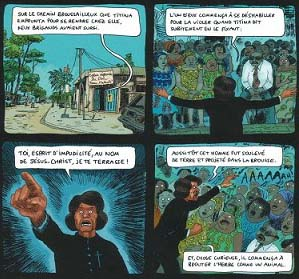
\includegraphics[width=\textwidth]{ChristologiePluraliste/Images/Aya.jpg}
 \caption{Aya de Yopougon, exemple des églises africaines proposant la guérison}
\end{marginfigure}
\begin{Ex}[Eglises africaines]
    marchent car elles proposent la guérison. 
    Approche néanmoins souvent trop individualisme

   
\end{Ex}

\subsection{La christologie à l’épreuve du dialogue}

\paragraph{Remet en cause le Christ comme le tout} Elle reinterpréte la différence entre contingent et absolu, Jésus et le Christ. On a bcp insisté sur \textit{Jésus et l'unique}. Si on annonce Jésus absolu, on ne peut entrer en dialogue. Il convient donc de se reposer la question de décentrer \textit{Jésus} par rapport à \textit{Dieu}. 

\paragraph{comment annoncer le Christ de manière dialogale et rassembler les hommes} question pas simple 
\begin{quote}
    Mgr Ladaria dans la présentation du document de la CTI (dont il est le secrétaire)
Christianisme et les religions 1996 écrit : « En contraste avec l’intention et la lettre même des textes conciliaires, un certain relativisme religieux s’est développé dans certains milieux au cours des années postconciliaires, comme si toutes les religions étaient d’égale valeur pour obtenir le salut; on perdit ainsi grandement le zèle missionnaire, et même la médiation unique
et universelle du Christ fut mise en doute. »
\end{quote}



\subsection{La christologie au défi de la fécondité sociale} 


\paragraph{fécondité} Les fruits de Sainteté. 
    Voir les critères de vérité de la Révélation :
\begin{quote}
 le GRIC \sn{GROUPE DE RECHERCHE
ISLAMO-CHRETIEN (GRIC), « L’Ecriture des uns vue par la foi des autres », Ces Ecritures
qui nous questionnent, la Bible et le Coran, Le Centurion, Paris, 1987, p. 71-139 (chapitre 3 ).}, 
Outre le contenu du message (du Coran), le Gric propose le critère de la fécondité du message
pour juger de l’authenticité de la révélation coranique. « L’autre critère (…) est celui de la
fécondité du message parmi les hommes (…). On doit donc pouvoir reconnaître dans la vie
individuelle et collective des hommes d’hier et d’aujourd’hui l’influence du message ; ce
qu’on pourrait appeler des fruits de sainteté » (p.103).
\end{quote}

\paragraph{Christologie} dans cette perspective. Quel image d'un Christ qui transforme notre société ? \textbf{des christo-praxies}. Certains auteurs montrent que le Christ doit inspirer notre agir et susciter la fraternité entre nous. Si elle nous enferme sur nous mêmes, il y a un problème.

 










 

